\documentclass[12pt,a4paper]{article}
\usepackage[utf8]{inputenc}
\usepackage[english]{babel}
\usepackage{amsmath}
\usepackage{amsfonts}
\usepackage{amssymb}
\usepackage{graphicx}
\usepackage{tikz}
\usepackage{pgfplots}
\usepackage{geometry}
\usepackage{fancyhdr}
\usepackage{listings}
\usepackage{xcolor}
\usepackage{hyperref}
\usepackage{booktabs}
\usepackage{caption}
\usepackage{subcaption}

% TikZ libraries
\usetikzlibrary{shapes,arrows,positioning,fit,backgrounds}

% Page geometry
\geometry{margin=2.5cm}

% Header and footer
\pagestyle{fancy}
\fancyhf{}
\rhead{TI0162 - IoT Project Documentation}
\lhead{ESP32-C3 Modular IoT System}
\cfoot{\thepage}

% Code listing settings
\lstset{
    language=Rust,
    backgroundcolor=\color{gray!10},
    basicstyle=\ttfamily\footnotesize,
    keywordstyle=\color{blue}\bfseries,
    commentstyle=\color{green!60!black},
    stringstyle=\color{red},
    numbers=left,
    numberstyle=\tiny\color{gray},
    stepnumber=1,
    numbersep=5pt,
    frame=single,
    rulecolor=\color{black!30},
    breaklines=true,
    showstringspaces=false,
    tabsize=2
}

% Hyperref setup
\hypersetup{
    colorlinks=true,
    linkcolor=blue,
    filecolor=magenta,
    urlcolor=cyan,
    citecolor=green,
    pdftitle={ESP32-C3 IoT System Technical Documentation},
    pdfauthor={Marcelo Correa},
    pdfsubject={Internet of Things Project - TI0162},
    pdfkeywords={ESP32-C3, IoT, Rust, Embassy, BME280, MQTT, WiFi}
}

% Document information
\title{
    \textbf{ESP32-C3 Modular IoT System} \\
    \large Technical Documentation \\
    \normalsize TI0162 - Internet of Things Project
}
\author{Marcelo Correa \\ \texttt{mvcorrea@gmail.com}}
\date{\today}

\begin{document}

\maketitle

\begin{abstract}
This document presents the technical documentation for a complete IoT system developed for ESP32-C3 microcontroller using Rust programming language and the Embassy async framework. The system implements a modular architecture for environmental data collection via BME280 sensor, WiFi connectivity, MQTT communication, and interactive serial console interface. The project demonstrates embedded systems development best practices with asynchronous programming, real-time data processing, and industrial IoT communication protocols. Future extensions include PID-controlled PWM devices for environmental control applications.
\end{abstract}

\tableofcontents
\newpage

\section{Introduction}

\subsection{Project Overview}
The ESP32-C3 Modular IoT System is a comprehensive embedded solution designed for environmental monitoring and control applications. Built using Rust programming language and the Embassy async framework, the system provides a robust, scalable platform for IoT deployments.

\subsection{Key Features}
\begin{itemize}
    \item \textbf{Modular Architecture}: Independent modules for sensor, connectivity, and communication
    \item \textbf{Asynchronous Processing}: Embassy framework for non-blocking operations
    \item \textbf{Real-time Communication}: MQTT protocol for industrial IoT integration
    \item \textbf{Interactive Console}: USB Serial/JTAG interface for configuration and monitoring
    \item \textbf{Environmental Sensing}: BME280 sensor for temperature, humidity, and pressure
    \item \textbf{Wireless Connectivity}: WiFi with automatic reconnection and DHCP
\end{itemize}

\subsection{Target Applications}
\begin{itemize}
    \item Environmental monitoring systems
    \item Smart building automation
    \item Industrial process monitoring
    \item Agricultural IoT solutions
    \item Research and educational platforms
\end{itemize}

\section{System Architecture}

\subsection{Hardware Platform}
The system is built around the ESP32-C3 microcontroller, specifically targeting the WeAct ESP32-C3 development board. The ESP32-C3 features:

\begin{itemize}
    \item RISC-V single-core processor at 160 MHz
    \item 400 KB SRAM, 384 KB ROM
    \item WiFi 802.11 b/g/n support
    \item Built-in USB Serial/JTAG controller
    \item 22 programmable GPIOs
    \item Multiple communication interfaces (I2C, SPI, UART)
\end{itemize}

\subsection{Software Architecture}

The system follows a modular architecture with clear separation of concerns. Each module is independently developed, tested, and maintained, allowing for easy extension and modification.

\begin{figure}[h!]
\centering
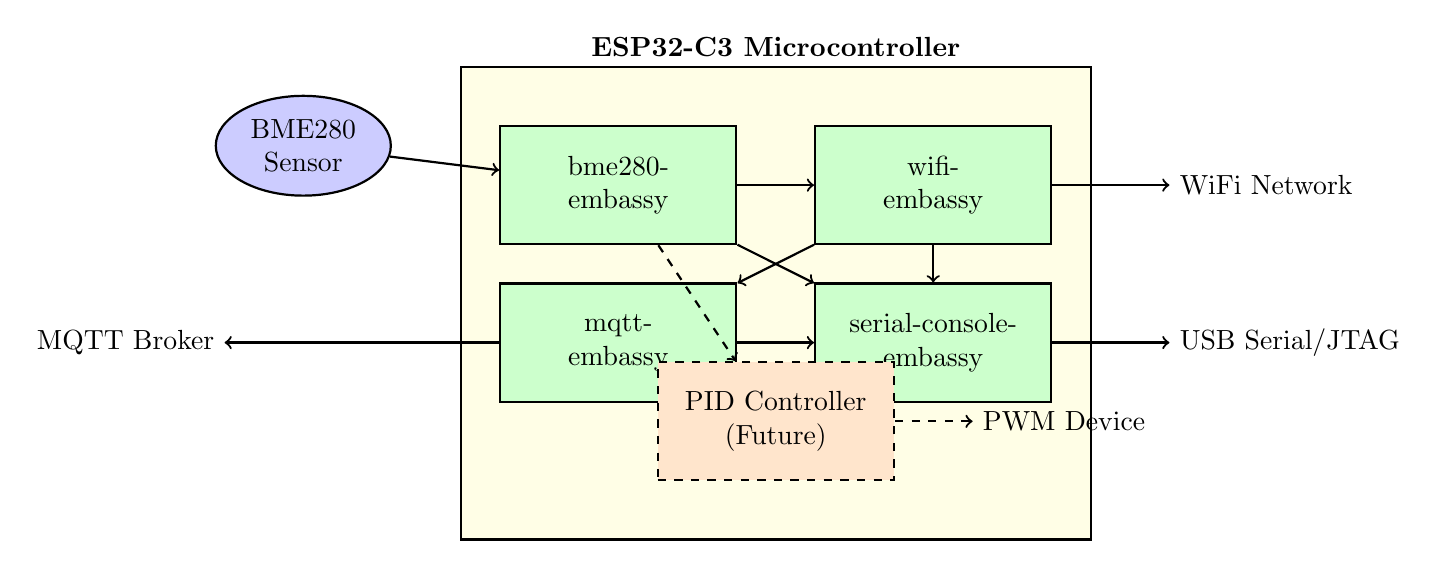
\begin{tikzpicture}[
    box/.style={rectangle, draw, thick, minimum width=3cm, minimum height=1.5cm, align=center},
    sensor/.style={ellipse, draw, thick, minimum width=2cm, minimum height=1cm, align=center, fill=blue!20},
    module/.style={box, fill=green!20},
    arrow/.style={->, thick}
]

% External sensor
\node[sensor] (bme280) at (0, 4) {BME280\\Sensor};

% ESP32-C3 main container
\node[box, minimum width=8cm, minimum height=6cm, fill=yellow!10] (esp32) at (6, 2) {};
\node[above] at (esp32.north) {\textbf{ESP32-C3 Microcontroller}};

% Internal modules
\node[module] (bme280mod) at (4, 3.5) {bme280-\\embassy};
\node[module] (wifi) at (8, 3.5) {wifi-\\embassy};
\node[module] (mqtt) at (4, 1.5) {mqtt-\\embassy};
\node[module] (console) at (8, 1.5) {serial-console-\\embassy};

% Future PID module (dashed)
\node[box, dashed, fill=orange!20] (pid) at (6, 0.5) {PID Controller\\(Future)};

% Data flow arrows
\draw[arrow] (bme280) -- (bme280mod);
\draw[arrow] (bme280mod) -- (wifi);
\draw[arrow] (wifi) -- (mqtt);
\draw[arrow] (bme280mod) -- (console);
\draw[arrow] (wifi) -- (console);
\draw[arrow] (mqtt) -- (console);

% Future PID connections (dashed)
\draw[arrow, dashed] (bme280mod) -- (pid);
\draw[arrow, dashed] (pid) -- (8.5, 0.5) node[right] {PWM Device};

% External connections
\draw[arrow] (mqtt) -- (-1, 1.5) node[left] {MQTT Broker};
\draw[arrow] (wifi) -- (11, 3.5) node[right] {WiFi Network};
\draw[arrow] (console) -- (11, 1.5) node[right] {USB Serial/JTAG};

\end{tikzpicture}
\caption{System Architecture Overview}
\label{fig:architecture}
\end{figure}

\subsection{Module Description}

\subsubsection{bme280-embassy Module}
Handles asynchronous communication with the BME280 environmental sensor via I2C interface. Provides:
\begin{itemize}
    \item Temperature reading (-40°C to +85°C)
    \item Humidity measurement (0-100\% RH)
    \item Atmospheric pressure (300-1100 hPa)
    \item Automatic calibration coefficient application
    \item Real-time data acquisition at configurable intervals
\end{itemize}

\subsubsection{wifi-embassy Module}
Manages WiFi connectivity with robust error handling and automatic reconnection:
\begin{itemize}
    \item WPA2/WPA3 security support
    \item DHCP client for automatic IP configuration
    \item Connection monitoring and automatic recovery
    \item Network stack integration for TCP/UDP operations
    \item Signal strength monitoring
\end{itemize}

\subsubsection{mqtt-embassy Module}
Implements MQTT 3.1.1 client for industrial IoT communication:
\begin{itemize}
    \item QoS 0 message publishing
    \item JSON-formatted sensor data transmission
    \item Configurable broker connection parameters
    \item Automatic reconnection on network failures
    \item Heartbeat and system status reporting
\end{itemize}

\subsubsection{serial-console-embassy Module}
Provides interactive console interface via USB Serial/JTAG:
\begin{itemize}
    \item Real-time system configuration
    \item WiFi credential management
    \item MQTT broker configuration
    \item System status monitoring
    \item Command-line interface with help system
\end{itemize}

\section{Hardware Configuration}

\subsection{Pin Assignment}

The system uses the following GPIO pin configuration:

\begin{table}[h!]
\centering
\begin{tabular}{@{}lll@{}}
\toprule
\textbf{Function} & \textbf{GPIO Pin} & \textbf{Description} \\
\midrule
I2C SDA & GPIO8 & BME280 data line \\
I2C SCL & GPIO9 & BME280 clock line \\
Status LED & GPIO3 & System status indicator \\
UART TX & GPIO21 & Serial console (alternative) \\
UART RX & GPIO20 & Serial console (alternative) \\
USB D+ & Built-in & USB Serial/JTAG data+ \\
USB D- & Built-in & USB Serial/JTAG data- \\
\bottomrule
\end{tabular}
\caption{GPIO Pin Assignment}
\label{tab:gpio}
\end{table}

\subsection{BME280 Connection}

\begin{figure}[h!]
\centering
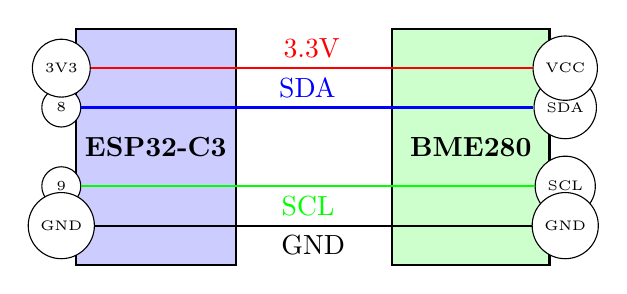
\begin{tikzpicture}[
    chip/.style={rectangle, draw, thick, minimum width=2cm, minimum height=3cm, align=center},
    pin/.style={circle, draw, fill=white, minimum size=0.3cm},
    wire/.style={thick}
]

% ESP32-C3
\node[chip, fill=blue!20] (esp32) at (0, 0) {\textbf{ESP32-C3}};
\node[pin] (sda) at (-1.2, 0.5) {\tiny 8};
\node[pin] (scl) at (-1.2, -0.5) {\tiny 9};
\node[pin] (vcc) at (-1.2, 1) {\tiny 3V3};
\node[pin] (gnd) at (-1.2, -1) {\tiny GND};

% BME280
\node[chip, fill=green!20] (bme280) at (4, 0) {\textbf{BME280}};
\node[pin] (bme_sda) at (5.2, 0.5) {\tiny SDA};
\node[pin] (bme_scl) at (5.2, -0.5) {\tiny SCL};
\node[pin] (bme_vcc) at (5.2, 1) {\tiny VCC};
\node[pin] (bme_gnd) at (5.2, -1) {\tiny GND};

% Connections
\draw[wire, red] (vcc) -- (bme_vcc) node[midway, above] {3.3V};
\draw[wire, black] (gnd) -- (bme_gnd) node[midway, below] {GND};
\draw[wire, blue] (sda) -- (bme_sda) node[midway, above] {SDA};
\draw[wire, green] (scl) -- (bme_scl) node[midway, below] {SCL};

\end{tikzpicture}
\caption{BME280 Sensor Connection Diagram}
\label{fig:bme280_connection}
\end{figure}

\section{Software Implementation}

\subsection{Development Environment}

The project is developed using:
\begin{itemize}
    \item \textbf{Rust 2021 Edition}: Modern systems programming language
    \item \textbf{Embassy Framework}: Async runtime for embedded systems
    \item \textbf{esp-hal}: Hardware Abstraction Layer for ESP32-C3
    \item \textbf{probe-rs}: Debugging and flashing tool
    \item \textbf{RTT (Real-Time Transfer)}: Debug output mechanism
\end{itemize}

\subsection{Key Dependencies}

\begin{lstlisting}[caption={Core Dependencies (Cargo.toml)}]
[dependencies]
# ESP32-C3 Hardware Abstraction Layer
esp-hal = { version = "1.0.0-rc.0", features = ["esp32c3", "unstable"] }
esp-hal-embassy = { version = "0.9.0", features = ["esp32c3"] }

# Embassy Async Framework
embassy-executor = { version = "0.7", features = ["task-arena-size-32768"] }
embassy-time = { version = "0.4" }
embassy-sync = { version = "0.7" }

# Communication and I/O
embedded-io-async = "0.6"
heapless = "0.8"

# Debugging
rtt-target = "0.5"
panic-rtt-target = "0.1"
\end{lstlisting}

\subsection{Module Integration Pattern}

Each module follows a consistent pattern for integration:

\begin{lstlisting}[caption={Module Integration Example}]
use embassy_executor::Spawner;
use embassy_time::{Duration, Timer};

#[embassy_executor::task]
async fn sensor_task() {
    let mut bme280 = BME280::new().await;
    
    loop {
        match bme280.read_all().await {
            Ok(data) => {
                rprintln!("Temperature: {:.2}°C", data.temperature);
                rprintln!("Humidity: {:.2}%", data.humidity);
                rprintln!("Pressure: {:.2} hPa", data.pressure);
            }
            Err(e) => rprintln!("Sensor error: {:?}", e),
        }
        
        Timer::after(Duration::from_secs(30)).await;
    }
}

#[esp_hal::main]
async fn main(spawner: Spawner) {
    // Initialize hardware and spawn tasks
    spawner.spawn(sensor_task()).ok();
    
    // Main loop
    loop {
        Timer::after(Duration::from_secs(1)).await;
    }
}
\end{lstlisting}

\section{Data Flow and Communication}

\subsection{MQTT Message Format}

The system publishes sensor data in JSON format:

\begin{lstlisting}[language=json, caption={Sensor Data Message}]
{
    "timestamp": "2025-01-15T10:30:00Z",
    "sensor": "BME280",
    "data": {
        "temperature": 23.5,
        "humidity": 65.2,
        "pressure": 1013.25
    },
    "metadata": {
        "device_id": "esp32-c3-001",
        "firmware_version": "1.0.0",
        "uptime": 3600
    }
}
\end{lstlisting}

\subsection{System Status Messages}

\begin{lstlisting}[language=json, caption={System Status Message}]
{
    "status": "online",
    "uptime": 7200,
    "free_heap": 45000,
    "wifi_rssi": -42,
    "sensor_status": "active",
    "mqtt_status": "connected"
}
\end{lstlisting}

\section{Future Enhancements}

\subsection{PID Control System}

The architecture is designed to support future integration of PID (Proportional-Integral-Derivative) controllers for environmental control applications.

\begin{figure}[h!]
\centering
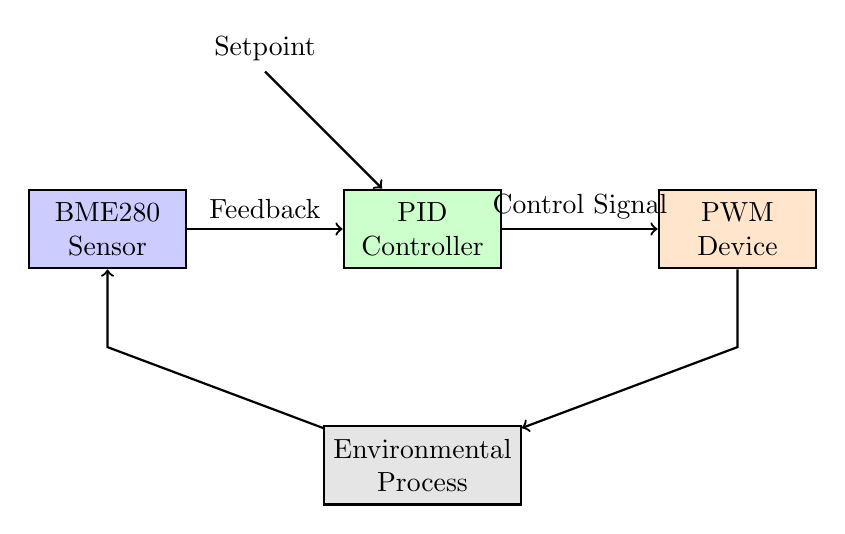
\begin{tikzpicture}[
    block/.style={rectangle, draw, thick, minimum width=2cm, minimum height=1cm, align=center},
    arrow/.style={->, thick}
]

% PID Control Loop
\node[block, fill=blue!20] (sensor) at (0, 0) {BME280\\Sensor};
\node[block, fill=green!20] (pid) at (4, 0) {PID\\Controller};
\node[block, fill=orange!20] (actuator) at (8, 0) {PWM\\Device};

% Process
\node[block, fill=gray!20] (process) at (4, -3) {Environmental\\Process};

% Arrows
\draw[arrow] (sensor) -- (pid) node[midway, above] {Feedback};
\draw[arrow] (pid) -- (actuator) node[midway, above] {Control Signal};
\draw[arrow] (actuator) -- (8, -1.5) -- (process);
\draw[arrow] (process) -- (0, -1.5) -- (sensor);

% Setpoint
\draw[arrow] (2, 2) node[above] {Setpoint} -- (pid);

\end{tikzpicture}
\caption{Planned PID Control Loop Integration}
\label{fig:pid_control}
\end{figure}

The PID controller will implement the standard control algorithm:

\begin{equation}
u(t) = K_p e(t) + K_i \int_0^t e(\tau) d\tau + K_d \frac{de(t)}{dt}
\end{equation}

Where:
\begin{itemize}
    \item $u(t)$ is the control output
    \item $e(t)$ is the error signal (setpoint - measured value)
    \item $K_p$, $K_i$, $K_d$ are the proportional, integral, and derivative gains
\end{itemize}

\subsection{Planned Features}

\begin{itemize}
    \item \textbf{Environmental Control}: Temperature, humidity regulation
    \item \textbf{PWM Output}: Variable speed fans, heaters, actuators
    \item \textbf{Multi-zone Control}: Independent control of multiple zones
    \item \textbf{Web Interface}: Browser-based monitoring and configuration
    \item \textbf{Data Logging}: Historical data storage and analysis
    \item \textbf{Alarm System}: Threshold-based alerts and notifications
\end{itemize}

\section{Performance and Specifications}

\subsection{System Performance}

\begin{table}[h!]
\centering
\begin{tabular}{@{}ll@{}}
\toprule
\textbf{Parameter} & \textbf{Value} \\
\midrule
Sensor Reading Interval & 30 seconds \\
MQTT Publish Rate & 30 seconds \\
WiFi Reconnection Time & < 10 seconds \\
Console Response Time & < 100 ms \\
Memory Usage & < 200 KB \\
Power Consumption & < 100 mA @ 3.3V \\
\bottomrule
\end{tabular}
\caption{System Performance Specifications}
\label{tab:performance}
\end{table}

\subsection{Sensor Specifications}

\begin{table}[h!]
\centering
\begin{tabular}{@{}lll@{}}
\toprule
\textbf{Parameter} & \textbf{Range} & \textbf{Accuracy} \\
\midrule
Temperature & -40°C to +85°C & ±0.5°C \\
Humidity & 0 to 100\% RH & ±3\% RH \\
Pressure & 300 to 1100 hPa & ±1 hPa \\
\bottomrule
\end{tabular}
\caption{BME280 Sensor Specifications}
\label{tab:sensor_specs}
\end{table}

\section{Conclusion}

The ESP32-C3 Modular IoT System represents a comprehensive solution for environmental monitoring and control applications. The modular architecture, combined with modern Rust programming practices and the Embassy async framework, provides a robust foundation for industrial IoT deployments.

The system's design emphasizes:
\begin{itemize}
    \item \textbf{Modularity}: Easy to extend and modify
    \item \textbf{Reliability}: Robust error handling and recovery
    \item \textbf{Performance}: Efficient async processing
    \item \textbf{Maintainability}: Clear code structure and documentation
    \item \textbf{Scalability}: Designed for future enhancements
\end{itemize}

Future developments will focus on expanding the control capabilities with PID algorithms and additional sensor integration, making this platform suitable for a wide range of industrial and commercial applications.

\section{References}

\begin{enumerate}
    \item ESP32-C3 Technical Reference Manual, Espressif Systems
    \item BME280 Environmental Sensor Datasheet, Bosch Sensortec
    \item Embassy Framework Documentation, \url{https://embassy.dev}
    \item MQTT Version 3.1.1 Specification, OASIS Standard
    \item Rust Programming Language Documentation, \url{https://doc.rust-lang.org}
    \item PID Control Theory, \url{https://en.wikipedia.org/wiki/Proportional-integral-derivative_controller}
\end{enumerate}

\appendix

\section{Build Instructions}

\subsection{Prerequisites}
\begin{lstlisting}[language=bash, caption={Development Environment Setup}]
# Install Rust
curl --proto '=https' --tlsv1.2 -sSf https://sh.rustup.rs | sh

# Add ESP32-C3 target
rustup target add riscv32imc-unknown-none-elf

# Install probe-rs
cargo install probe-rs --features cli

# Clone repository
git clone <repository-url>
cd workspace
\end{lstlisting}

\subsection{Building and Flashing}
\begin{lstlisting}[language=bash, caption={Build and Flash Commands}]
# Build individual modules
cd bme280-embassy
cargo build --release

cd ../wifi-embassy  
cargo build --release

cd ../mqtt-embassy
cargo build --release

cd ../serial-console-embassy
cargo run --example direct_usb_console --release
\end{lstlisting}

\section{Configuration Files}

\subsection{Environment Configuration}
\begin{lstlisting}[caption={.cargo/config.toml}]
[env]
WIFI_SSID = "YourNetworkName"
WIFI_PASSWORD = "YourPassword"
MQTT_BROKER_IP = "192.168.1.100"
MQTT_BROKER_PORT = "1883"
MQTT_CLIENT_ID = "esp32-c3-device"
MQTT_TOPIC_PREFIX = "esp32"
\end{lstlisting}

\end{document}